
\chapter{Requirements}
\label{chap:requirements}

%\section{Introduction}
%\label{sec:workflowexample}

This chapter specifies the requirements of the system.  

...




\section{High-level Requirements}
\label{sec:requirements}

...

Figure~\ref{fig:highlevelview} depicts the high-level view of
data flow through the system. 

...

%Through sample groups, users can share data with each other.

% convert highlevelview2.png highlevelview2.pdf

\begin{figure}[!htpb]
  \centering
  \includegraphics[width=.8\textwidth]{diagrams/System}
  \caption{High-level view of system functionality}
  \label{fig:highlevelview}
\end{figure}



\section{System Functionality}
\label{sec:systemfunction}

This section describes in detail the main features and capabilities of
the system. The Glossary appendix (Appendix~\ref{main}) 
describes the important domain concepts.




%%% Local Variables: 
%%% mode: latex
%%% TeX-master: "main"
%%% End: 
